\chapter{Introduction}
\label{chapter:introduction}

The Steiner Multicycle Problem (\(\steinercycle\)) was introduced by \cite{Pereira2018TheSM} in the context of vehicle routing where multiple companies must visit pickup and delivery locations. That way, a group of companies can collaborate to realize the necessary deliveries and reduce the total cost of transportation. 
Notably, one assumes that the companies must make the deliveries periodically, and the size of each delivery is much smaller than the vehicles' capacities.
The interested reader may find more details about this application in \cite{Pereira2018TheSM}.

The problem \(\steinercycle\) has as input an undirected graph \(G\), a function $c \colon E(G) \to \mathbb{R}_\ge$ that associates a cost to each edge of \(G\), and a set \(\{T_1, \dots, T_k\}\) of pairwise disjoint subsets of vertices of \(G\) (a.k.a. \textbf{terminal sets}). The goal of the problem is to find a minimum-cost set of cycles \(\mathcal{C}\), such that each terminal set \(T_i\) is contained within the same cycle.

A solution to the Steiner Multicycle Problem can be represented by a single multiset that contains all the edges forming the cycles in the solution. Moreover, since a multiset of edges and the cycles induced by these edges are equivalent, throughout this work, we refer to the solution as both the multiset of edges and the subgraph of \(G\) induced by those edges interchangeably.

The solution cost is defined as the sum of all associated costs of the edges in the solution multiset.

The problem is defined next. An instance of \(\steinercycle\) and a feasible solution are depicted in Figure~\ref{fig:exem_multicycle}.

\medskip
\noindent \fbox{
	\parbox{.97\textwidth}{
		\noindent
		\textsc{Steiner Multicycle Problem (\textbf{SMCP})}\\
		\noindent
		\textbf{Instance}: A graph \(G\), $c \colon E(G) \to \mathbb{R}_\ge$, and a set \(\{T_1, \dots, T_k\}\) of pairwise disjoint subset of vertices of \(G\) (i.e. the terminals).\\
		%\noindent
		%\textbf{Parameter}: $k$.
		\noindent
		\textbf{Goal}: Find in \(G\) a minimum cost set of cycles such that all terminals in \(T_i\) belong to the same cycle, for each \(i \in [k]\).
	}
}
\medskip

\begin{figure}[H]
    \centering
\begin{tikzpicture}

\Vertex[x=0, y=2, label=$t'_3$, color=white]{A}
\Vertex[label=$t'_2$, color=white]{B}
\Vertex[x=2, y=2, color=white]{C}
\Vertex[x=2, y=0, color=white]{D}
\Vertex[x=2, y=4, label=$t_2$, color=white]{E}
\Vertex[x=4, y=2, label=$t_3$, color=white]{F}
\Vertex[x=4, y=0, color=white]{G}
\Vertex[x=6, y=2, label=$t_1$, color=white]{H}
\Vertex[x=6, y=0, label=$t'_1$, color=white]{I}

\Edge[lw=3pt, label=$e_1$, position=left](A)(B)
\Edge[lw=4pt, label=$e_2$, position=above](A)(C)
\Edge[lw=4pt, label=$e_3$, position=above](B)(D)
\Edge[lw=4pt, label=$e_4$, position=left](C)(D)
\Edge[lw=4pt, label=$e_5$, position=left](C)(E)
\Edge[lw=4pt, label=$e_6$, position=above](C)(F)
\Edge[label=$e_7$, position=above left](D)(F)
\Edge[label=$e_8$, position=above](D)(G)
\Edge[lw=4pt, label=$e_9$, position=above right](E)(F)
\Edge[lw=4pt, label=$e_{10}$, position=above](G)(I)
\Edge[lw=4pt, label=$e_{11}$, position=above left](G)(H)

\end{tikzpicture}
    \caption{An example of a feasible solution for the \(\steinercycle\) considering the set of pairs of terminals \(\{\{t_1, t'_1\}, \{t_2, t'_2\}, \{t_3, t' _3\}\}\). The solution is represented by the edges in bold and corresponds to the multiset \(\{e_1, e_2, e_3, e_4, e_5, e_6, e_9, e_{10}, e_{11}, e_{10}, e_{11}\}\). The weights of the edges were omitted for simplicity.}
    \label{fig:exem_multicycle}
\end{figure}

\cite{Pereira2018TheSM} studied the problem for complete metric graphs (i.e., complete graphs that guarantee the triangular inequality for the edges costs). The authors presented a 4-approximation algorithm, a heuristic algorithm, and a mixed-integer linear formulation for the problem.
Moreover, the authors performed computational experiments comparing the proposed heuristic, called \textit{Refinement Search}, to a GRASP implementation. In summary, the results showed that the proposed heuristic reached better quality results in less time.

\citeauthor{Pereira2018TheSM} also introduced a restricted version of the Steiner Multicycle Problem (R-\(\steinercycle\)) in which every terminal set has only two vertices, one for pickup and the other for delivery. \cite{LINTZMAYER2020134} showed an equivalence between the two problems -- \(\steinercycle\) and R-\(\steinercycle\) -- by proposing a simple transformation from instances of the \(\steinercycle\) to R-\(\steinercycle\), which we present below. 

Let \(\mathcal{T} = \{t_1, \dots, t_\ell\}\) be a set of terminals, and create \(\ell\) new vertices \(\{u_1, \dots, u_\ell\}\). For each \(i \in \{1, \ldots, \ell\}\), we create an edge \(\{t_i, u_i\}\) of cost zero. We define \(\{\{u_1, t_2\}, \dots, \{u_{\ell-1}, t_\ell\}, \{u_\ell, t_1\}\}\) as terminals pairs of an instance of R-\(\steinercycle\). Note that the set of edges that forms a solution of \(\steinercycle\) with terminals of \(\mathcal{T}\) have the same cost of a solution of R-\(\steinercycle\) after the addition of the new vertices. Given that equivalence, throughout this work, we assume that each terminal set in the \(\steinercycle\) contains exactly two vertices; i.e., we will refer to the R-SMCP as SMCP and denote terminal sets as terminal pairs.

\cite{smcp_3apx} proposed a 3-approximation for complete metric graphs, which is based on a 2-approximation for the Survivable Network Design Problem and the concept of T-joins, a generalization of the well-known perfect matching. This algorithm is inspired by the results obtained for the metric Travelling Salesman Problem (TSP) by \cite{Christofides2022WorstCaseAO}.

It is also essential to notice that, even for the restricted case, the Steiner Multicycle Problem is \(\nonpoly\)-hard. This can be verified by reducing the TSP to the R-\(\steinercycle\) using a strategy similar to the one presented by \citeauthor{LINTZMAYER2020134}.

This work proposes a \textbf{polynomial-time approximation scheme} (PTAS) for the \(\steinercycle\) on a special class of graphs called \textit{bounded genus graphs}, a generalization of the well-known class of planar graphs.

This work is structured as follows. Chapter~\ref{chapter:definitions} introduces some basic definitions in Graph Theory and Approximation Algorithms, as well as some definitions used to present and prove the results of this work. Chapter~\ref{chapter:related_work} overviews the literature for \(\steinercycle\) and related problems. Chapters~\ref{chapter:pc-partition} and~\ref{chapter:spanner} introduce some tooling necessary for achieving the PTAS. Next, Section~\ref{section:ptas_bounded_tree} of Chapter~\ref{chapter:apx_schemes_for_smcp} proves a PTAS for bounded treewidth graphs, which is an essential result to prove the PTAS for bounded genus graphs in the Section~\ref{section:ptas_bounded_genus} of the same chapter. Chapter~\ref{chapter:experiments} presents some experimental results of the 3-approximation algorithm proposed by \cite{smcp_3apx}. Finally, Chapter~\ref{chapter:conclusion} delivers general remarks on this work and proposes possible paths for future work.

\section{Algorithm Overview}

As we shall see, the proposed PTAS for \steinercycle\ is inspired by the PTAS for the Steiner Tree Problem due to \cite{Bateni}. Put briefly, the proposed algorithm for \steinercycle\ consists of the following steps:

\begin{enumerate}
    \item The algorithm receives as input a graph \(G_{in}\) with bounded-genus, and a set \(\mathcal{D} = \{T_1, \dots, T_k\}\) of terminal pairs.

    \item It begins by creating a spanner subgraph (i.e., a subgraph whose size is bounded by a constant time \(\opt\) and has a valid solution with a cost at most \((1 + \epsilon) \opt\) of \(G_{in}\). This is done with an auxiliary clustering algorithm provided by Theorem~\ref{chapter:pc-partition}.
    
    \item The edges of the spanner are split into \(k\)-disjoint sets, then the edges in the smallest set are contracted. After the contraction, the algorithm applies \citeauthor{Demaine2010}'s Theorem (\cite{Demaine2010} Theorem~1.1) to convert the spanner subgraph to a bounded treewidth graph.

    \item A dynamic programming algorithm is used to solve the SMCP in the bounded treewidth graph generated in the previous step. During this process, the algorithm only considers a subset of the possible solutions that organize the set of unpaired terminals (from the bottom-up in the dynamic programming tree) in valid ways.

    \item Finally, it constructs the final solution, i.e., the PTAS for bounded genus, by leveraging the solution in bounded-treewidth and the set of edges contracted in the previous step.
\end{enumerate}